\documentclass[../design_doc.tex]{subfiles}
 
\begin{document}

\section{VOL Connector Design}

\subsection{Mapping HDF5 to DAOS}

The central paradigm for mapping \acrshort{hdf5} to \acrshort{daos} is that \acrshort{hdf5} files are stored as \acrshort{daos} containers, and \acrshort{hdf5} objects (groups, datasets, committed datatypes, and maps) are stored as \acrshort{daos} objects, both using a 1:1 mapping. All metadata and raw data associated with an \acrshort{hdf5} object is then stored as entries in the key value store associated with that object provided by \acrshort{daos}.

Since \acrshort{daos} containers are identified by a UUID, the \gls{connector} uses a hashing function to generate a UUID from the file name. Each container for an \acrshort{hdf5} file contains at least two objects: the global metadata object and the root group. The global metadata object stores metadata that describes properties that apply to the entire file. The root group is always the start of the \acrshort{hdf5} group structure, and uses the same format as all other groups.

Similar to the native \acrshort{hdf5} file format, the formats for the different object types are kept similar, with only differences as necessary to represent the specific object type. All object types have a creation property list and a reference count (not yet implemented) stored under the \mintcinline{/Internal Metadata} \gls{dkey} and the \mintcinline{Creation Property List} and \mintcinline{Reference Count} \glspl{akey}, respectively. The \mintcinline{/} prefix for the \mintcinline{/Internal Metadata} \gls{dkey} prevents conflicts with arbitrarily named \acrshort{hdf5} links, which cannot contain the \mintcinline{/} character.

\newpage

\subsubsection{Groups}

The purpose of \acrshort{hdf5} groups is to store links to other objects. Each link is stored under a \gls{dkey} equal to the link's name and under the constant \gls{akey} \mintcinline{Link}. Links can be hard links, in which case the value stored for the link is the object ID for the target object. This object ID can then be used to directly open the target object. Alternatively, links can be soft links, in which case the value stored for the link is the path name of the target object. Once retrieved, this path name must be traversed in order to open the target object.

When link creation order is tracked for a group, additional information is written to that group under the \mintcinline{/Link Creation Order} \gls{dkey}. Under that \gls{dkey}, link creation order-related information is stored under the following \glspl{akey}:

\begin{itemize}
    \item \mintcinline{Max Link Creation Order} --- This \gls{akey} stores the current maximum link creation order value for the group. The maximum link creation order value starts at 0 and increases as new links are created in the group. This value is mostly used to supply a group's maximum link creation order value when a call to \mintcinline{H5Gget_info(_by_name/_by_idx)} is made.
    \item \mintcinline{Num Links} --- This \gls{akey} stores the current number of links in the group.
    \item \mintcinline{<encoded num. links>} --- The value for this \gls{akey} is determined by encoding the current number of links in the group \textit{at creation time of the new link} into a binary buffer; this encoded value represents the creation order index value assigned to the new link being written. This \gls{akey} is used to store a mapping from link creation order index values to link names, which allows an easy lookup of a link's name by a given creation order index value. One of these \glspl{akey} will exist for each link currently in the group, as a new \gls{akey} will be added each time a new link is written to the group.
    \item \mintcinline{<encoded num. links>0} --- The value for this \gls{akey} is determined similarly to the previous \gls{akey}, but the \gls{akey} value is suffixed with a trailing \mintcinline{0} byte in order to distinguish it from the previous \gls{akey}. This \gls{akey} is used to store a mapping from link creation order index values to link targets, which allows an easy lookup of a link's target by a given creation order index value. One of these \glspl{akey} will exist for each link currently in the group, as a new \gls{akey} will be added each time a new link is written to the group.
\end{itemize}

%\todo{Update figure for creation order changes}
\begin{figure}
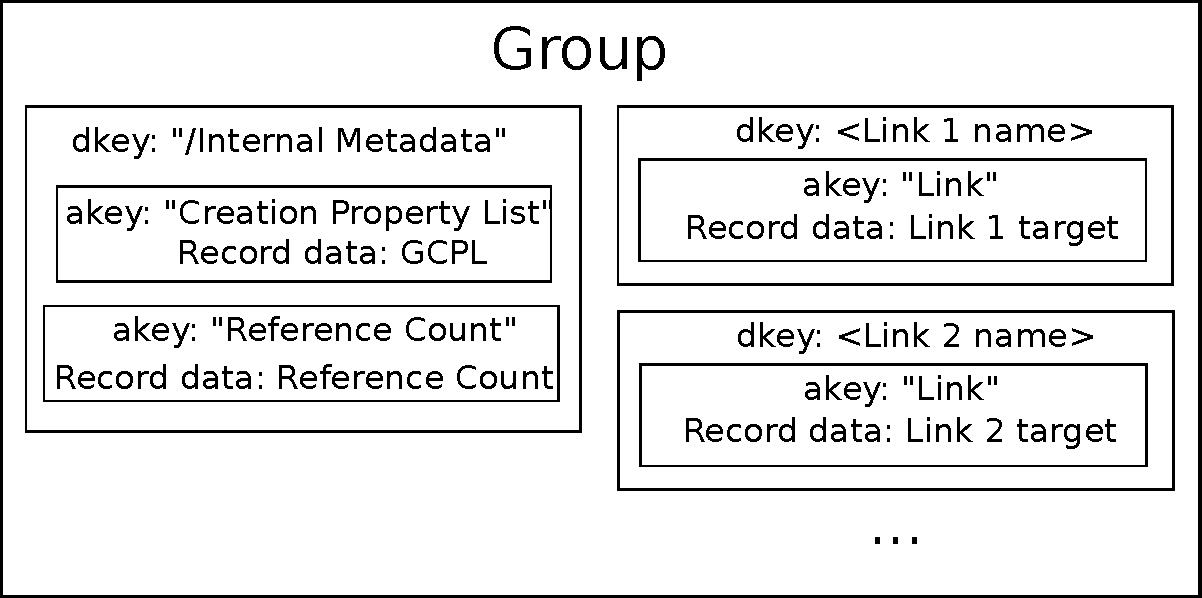
\includegraphics[width=0.6\textwidth]{group_figure}
\caption{Group dkey and link examples.}
\label{fig:group}
\end{figure}

\newpage

\subsubsection{Datasets}

Datasets are used to store the bulk array data in \acrshort{hdf5}. A dataset's metadata is stored under the \mintcinline{/Internal Metadata} \gls{dkey} and under the following \glspl{akey}:

\begin{itemize}
 \item \mintcinline{Datatype} --- This \gls{akey} stores the dataset's datatype.
 \item \mintcinline{Dataspace} --- This \gls{akey} stores the dataset's dataspace.
 \item \mintcinline{Creation Property List} --- This \gls{akey} stores the dataset's Dataset Creation Property List.
 \item \mintcinline{Fill Value} --- This optional \gls{akey} stores the dataset's fill value in file format.
\end{itemize}

A dataset's raw data is divided into ``chunks'' which are regularly spaced blocks of data, where the size of the block is specified by the application. Each data chunk is stored in its own \gls{dkey}, which is encoded with a leading 0 byte, followed by $<$number of dimensions$>$ 64-bit little endian unsigned integers which denote the chunk offset within the dataset. The \mintcinline{0} prefix for chunks prevents the binary chunk \glspl{dkey} from conflicting with the string metadata \gls{dkey}, since nonzero length strings cannot begin with 0 (\mintcinline{'\0'}).

For datasets with fixed-length datatypes, the data for a chunk is stored in a single \gls{akey} with a value of a 0 byte. The data is stored as an array of records, where each record corresponds to an element in the dataset. The record size is therefore equal to the size of the datatype and the number of records is equal to the number of elements in the data chunk. For datasets with variable-length datatypes, the fixed-length portion of the data is stored normally, but each variable-length sequence is stored separately in the global metadata object, with a \gls{dkey} consisting of a randomly generated UUID, and the constant \gls{akey} \mintcinline{Blob}. The UUID used for the \gls{dkey} for the variable-length sequence is stored in the fixed-length portion of the dataset. Reference type data is stored in the same manner as variable-length data.

Fill values are not written to the dataset's data array, rather, we take advantage of \acrshort{daos}' behaviour when reading from extents that have not been written to. In this case, \acrshort{daos} does not modify the sections of the read buffer that correspond to the missing records. In order to implement fill values, when the user reads from a dataset, we first propagate the fill value to the entire selection in the read buffer (or type conversion buffer if appropriate), then after fetching the data from \acrshort{daos}, any unwritten elements will contain the fill value.

%\todo{Add figure for variable-length datasets}
\begin{figure}

\includegraphics[width=0.6\textwidth]{dataset_figure}
\caption{Fixed length dataset dkey examples.}
\label{fig:dataset}
\end{figure}

\newpage

\subsubsection{Committed Datatypes}

A committed datatype is an \acrshort{hdf5} datatype that has been stored as an \acrshort{hdf5} object in the group structure. A committed datatype's metadata is stored under the \mintcinline{/Internal Metadata} \gls{dkey} and under the following \glspl{akey}:

\begin{itemize}
    \item \mintcinline{Datatype} --- This \gls{akey} stores the committed datatype's actual datatype.
    \item \mintcinline{Creation Property List} --- This \gls{akey} stores the committed datatype's Datatype Creation Property List.
\end{itemize}

%\todo{Add figure for committed datatype}

\newpage

\subsubsection{Attributes}

\acrshort{hdf5} attributes attached to an object (group, dataset, committed datatype or map object) are stored under that object's \mintcinline{/Attribute} \gls{dkey} (note that the \mintcinline{/} prefix for the \mintcinline{/Attribute} \gls{dkey} prevents conflicts with arbitrarily named \acrshort{hdf5} links, which cannot contain the \mintcinline{/} character). Under that \gls{dkey}, an attribute's metadata and raw data is stored under the following \glspl{akey}:

\begin{itemize}
 \item \mintcinline{T-<attribute name>} --- This \gls{akey} stores the attribute's datatype.
 \item \mintcinline{S-<attribute name>} --- This \gls{akey} stores the attribute's dataspace.
 \item \mintcinline{P-<attribute name>} --- This \gls{akey} stores the attribute's Attribute Creation Property List.
 \item \mintcinline{V-<attribute name>} --- This \gls{akey} stores the attribute's value.
\end{itemize}

When attribute creation order is tracked for an object, additional information is written to that object under the same \mintcinline{/Attribute} \gls{dkey} and under the following \glspl{akey}:

\begin{itemize}
 \item \mintcinline{Max Attribute Creation Order} --- This \gls{akey} stores the current maximum attribute creation order value for the object. The maximum attribute creation order value starts at 0 and increases as new attributes are added to the object.
 \item \mintcinline{Num Attributes} --- This \gls{akey} stores the current number of attributes attached to the object.
 \item \mintcinline{0<encoded num. attributes>} --- The value for this \gls{akey} is determined by encoding the current number of attributes attached to the object \textit{at creation time of the new attribute} into a binary buffer, prefixed with a leading \mintcinline{0} byte; this encoded value represents the creation order index value assigned to the new attribute being written. This \gls{akey} is used to store a mapping from attribute creation order index values to attribute names, which allows an easy lookup of an attribute's name by a given creation order index value. One of these \glspl{akey} will exist for each attribute currently attached to the object, as a new \gls{akey} will be added each time a new attribute is written to the object.
 \item \mintcinline{C-<attribute name>} --- This \gls{akey} stores the attribute's creation order value.
\end{itemize}

%\todo{Add figure for attributes + attribute creation order}

\newpage

\subsubsection{Object IDs}

%\todo{Update for \acrshort{daos} object ID allocator changes}

\acrshort{daos} objects are referenced through the \acrshort{daos} API by a 128 bit object ID. \acrshort{daos} reserves the upper 32 bits to encode its information, such as the object class. The second 32 bits are used by the application to encode its specific information, and the lower 64 bits are used as a unique object identifier. The lower 64 bits are generated using a \acrshort{daos} routine to allocate ID ranges for each process, with a separate range of IDs for objects created collectively. There are currently two reserved values for these lower 64 bits, 0 for the global metadata object, and 1 for the root group. The top 2 bits of the application information block are used to encode the \acrshort{hdf5} object type. This removes the need to store the object type in the key-value store for the object itself, and allows the \gls{connector} to determine the object type and therefore the routines used to access it without needing to query \acrshort{daos}, reducing the number of server requests needed for metadata operations. The entire 128 object ID is used as the "token" for the \acrshort{hdf5} token API, which is meant to replace the use of file addresses.

\end{document}
